%%%%%%%%%%%%%%%%%%%%%%%%%%%%%%%%%%%%%%%%%
% a0poster Landscape Poster
% LaTeX Template
% Version 1.0 (22/06/13)
%
% The a0poster class was created by:
% Gerlinde Kettl and Matthias Weiser (tex@kettl.de)
% 
% This template has been downloaded from:
% http://www.LaTeXTemplates.com
%
% License:
% CC BY-NC-SA 3.0 (http://creativecommons.org/licenses/by-nc-sa/3.0/)
%
%%%%%%%%%%%%%%%%%%%%%%%%%%%%%%%%%%%%%%%%%

%----------------------------------------------------------------------------------------
%	PACKAGES AND OTHER DOCUMENT CONFIGURATIONS
%----------------------------------------------------------------------------------------

\documentclass[a0,landscape]{a0poster}
\usepackage[export]{adjustbox}
\usepackage{multicol} % This is so we can have multiple columns of text side-by-side
\columnsep=100pt % This is the amount of white space between the columns in the poster
\columnseprule=3pt % This is the thickness of the black line between the columns in the poster

\usepackage[svgnames]{xcolor} % Specify colors by their 'svgnames', for a full list of all colors available see here: http://www.latextemplates.com/svgnames-colors

% \usepackage{times} % Use the times font
% \usepackage{palatino} % Uncomment to use the Palatino font
\usepackage{fontspec}
\setromanfont{Libre Baskerville}
\setsansfont{Open Sans}

\usepackage{graphicx} % Required for including images
\graphicspath{{figures/}} % Location of the graphics files
\usepackage{booktabs} % Top and bottom rules for table
\usepackage[font=small,labelfont=bf]{caption} % Required for specifying captions to tables and figures
\usepackage{amsfonts, amsmath, amsthm, amssymb} % For math fonts, symbols and environments
\usepackage{wrapfig} % Allows wrapping text around tables and figures
\usepackage{setspace}

\begin{document}

%----------------------------------------------------------------------------------------
%	POSTER HEADER 
%----------------------------------------------------------------------------------------

% The header is divided into three boxes:
% The first is 55% wide and houses the title, subtitle, names and university/organization
% The second is 25% wide and houses contact information
% The third is 19% wide and houses a logo for your university/organization or a photo of you
% The widths of these boxes can be easily edited to accommodate your content as you see fit

\begin{minipage}[b]{0.55\linewidth}
{\veryHuge\color{NavyBlue} \textbf{qc3C} \color{Black} \textit{-- Reference-free quality assessment \\ for Hi-C sequencing data}\par}
\vspace{1em}
\huge \textbf{Matthew Z. DeMaere\textsuperscript{*} \& Aaron E. Darling}\\ % Author(s)
\huge ithree institute -- University of Technology Sydney\\ % University/organization
\end{minipage}
%
\begin{minipage}[b]{0.25\linewidth}
\color{DarkSlateGray}\Large \textbf{Contact Information}\\
\texttt{matthew.demaere@uts.edu.au}\\ % Email address
\texttt{https://github.com/cerebis/qc3C}\\
\texttt{conda install -c cerebis qc3c}\\
\texttt{docker pull cerebis/qc3c:latest}\\
\end{minipage}
%
\begin{minipage}[b]{0.19\linewidth}
\adjustbox{center, raise=2cm}{
\includegraphics[width=15cm]{i3-logo-wider.png}}
\adjustbox{center, raise=1cm}{
\includegraphics[width=10cm]{uts-logo-trans.png}}
% Logo or a photo of you, adjust its dimensions here
\end{minipage}

% \vspace{1cm} % A bit of extra whitespace between the header and poster content

%----------------------------------------------------------------------------------------

\begin{multicols}{4} % This is how many columns your poster will be broken into, a poster with many figures may benefit from less columns whereas a text-heavy poster benefits from more

%----------------------------------------------------------------------------------------
%	INTRODUCTION
%----------------------------------------------------------------------------------------

\color{DarkSlateGray} % SaddleBrown color for the introduction

\section*{Introduction}

Hi-C is a high-throughput sequencing technique that captures genome-wide observations of DNA proximity interactions. To do so, the Hi-C protocol breaks and then rejoins DNA in such a way that chimeric fragments are generated whose ends derive from nonadjacent loci. Once purified and sequenced, read-pairs derived from each fragment can be used to identify the interacting loci through read-mapping. A by-product of breaking and rejoining DNA is the creation of a predictable sequence duplication artefact (DA) (fig. \ref{fig:junction}), left behind by the process of restriction digest, end-fill and re-ligation. After DNA shearing and size filtering, these proximity-ligation (PL) junctions can occur at any point along fragments which go on to sequencing. Read-through occurs when sequencing reads crossover a PL junction, the probability of which is a function of read and fragment length. 

The process of generating and then observing PL containing fragments (valid Hi-C pairs) can be inefficient. Many published Hi-C datasets are composed of <1\% valid Hi-C pairs, with the remainder effectively conventional shotgun data. Even so, the value of the information derived from Hi-C is such that any library may still be useful provided it is sequenced to sufficient depth. Knowing, then, the fraction of valid Hi-C pairs (the signal) prior to conducting a full sequencing run is an important detail, which can be obtained by way of a small pilot sequencing run and a quality analysis tool. 

Quality analysis tools have traditionally relied on a reference genome to assess Hi-C signal content, which is not always available. Here we introduce a means of reference-free assessment that builds upon the notion that PL events are likely to create $k$-mers that would not naturally occur in the sample. Using an empirical cumulative distribution of $k$-mer depths, our new algorithm computes the probability that a read containing a DA was generated by the PL reaction. This in turn enables the fraction of valid Hi-C pairs to be estimated. We characterise the accuracy of the new algorithm on simulated data and demonstrate the utility of QC reports generated from real datasets.

Both our reference-free and reference-based QC is available in qc3C, an easy to use open-source tool that integrates with the multiQC framework \cite{Ewels2016-up}. To our knowledge, qc3C is the first reference-free Hi-C quality assessment tool, enabling Hi-C to be more easily applied to non-model organisms and environmental samples.

%----------------------------------------------------------------------------------------
%	METHODS
%----------------------------------------------------------------------------------------

\section*{Method}

To assess the signal content from a sample Hi-C read-pairs alone, first a $k$-mer frequency database is constructed internally using Jellyfish \cite{Marcais2012-bc}, where $k$ is chosen to balance specificity against database size (e.g. $k=24$). Next, each read in the sample is searched for DAs. If one is found, its starting location defines an anchor position $x_i$, otherwise an anchor is drawn uniformly at random along the read $x_i \sim U(k, l_{read}-l_{junc}-k)$. From a sliding window $j \in [x_i-k:x+l_{junc}]$, $k$-mers are extracted either side and within the junction containing region and the count $c_{ij}$ for each $k$-mer is obtained from the database (fig. \ref{fig:junction}). An observation of local relative frequency about the anchor $x_i$ is then calculated as the ratio of geometric means (eqn \ref{fig:eq1}). A table of observations is subsequently constructed $T = (x_i, \lambda_i)$, where $\lambda_i$ is a binary indicator variable for the presence ($\lambda_i=1$) of the DA.

Bootstrapped estimates for the observed fraction of true DAs is obtained as follows. A random sample of size $n$ is taken from $T$ and reduced to a unique set by relative coverage $f^k_i$. In ascending $f^k_i$ order, empirical ranked p-values are assigned for observations where $\lambda_i=0$, these p-values are then distributed over the remaining observations where $\lambda_i=1$ and the fraction of observable Hi-C pairs is estimated by summing p-values when $\lambda_i=1$. Quantiles $q=[0.025, 0.975]$ are used to define a 95\% CI over the bootstrapped estimates. This 95\% CI is lastly adjusted to account for the portion of total fragment extent that was unobservable due to the difference in read vs fragment length.

\begin{minipage}{0.8\linewidth}\vspace{1cm}
\begin{equation}\label{fig:eq1}
f^k_i=\frac{GM({c_{ij} | j \in inner})}{GM({c_{ij} | j \in outer})}
\end{equation}
\end{minipage}

\begin{minipage}{\linewidth}
\begin{center}\vspace{1cm}
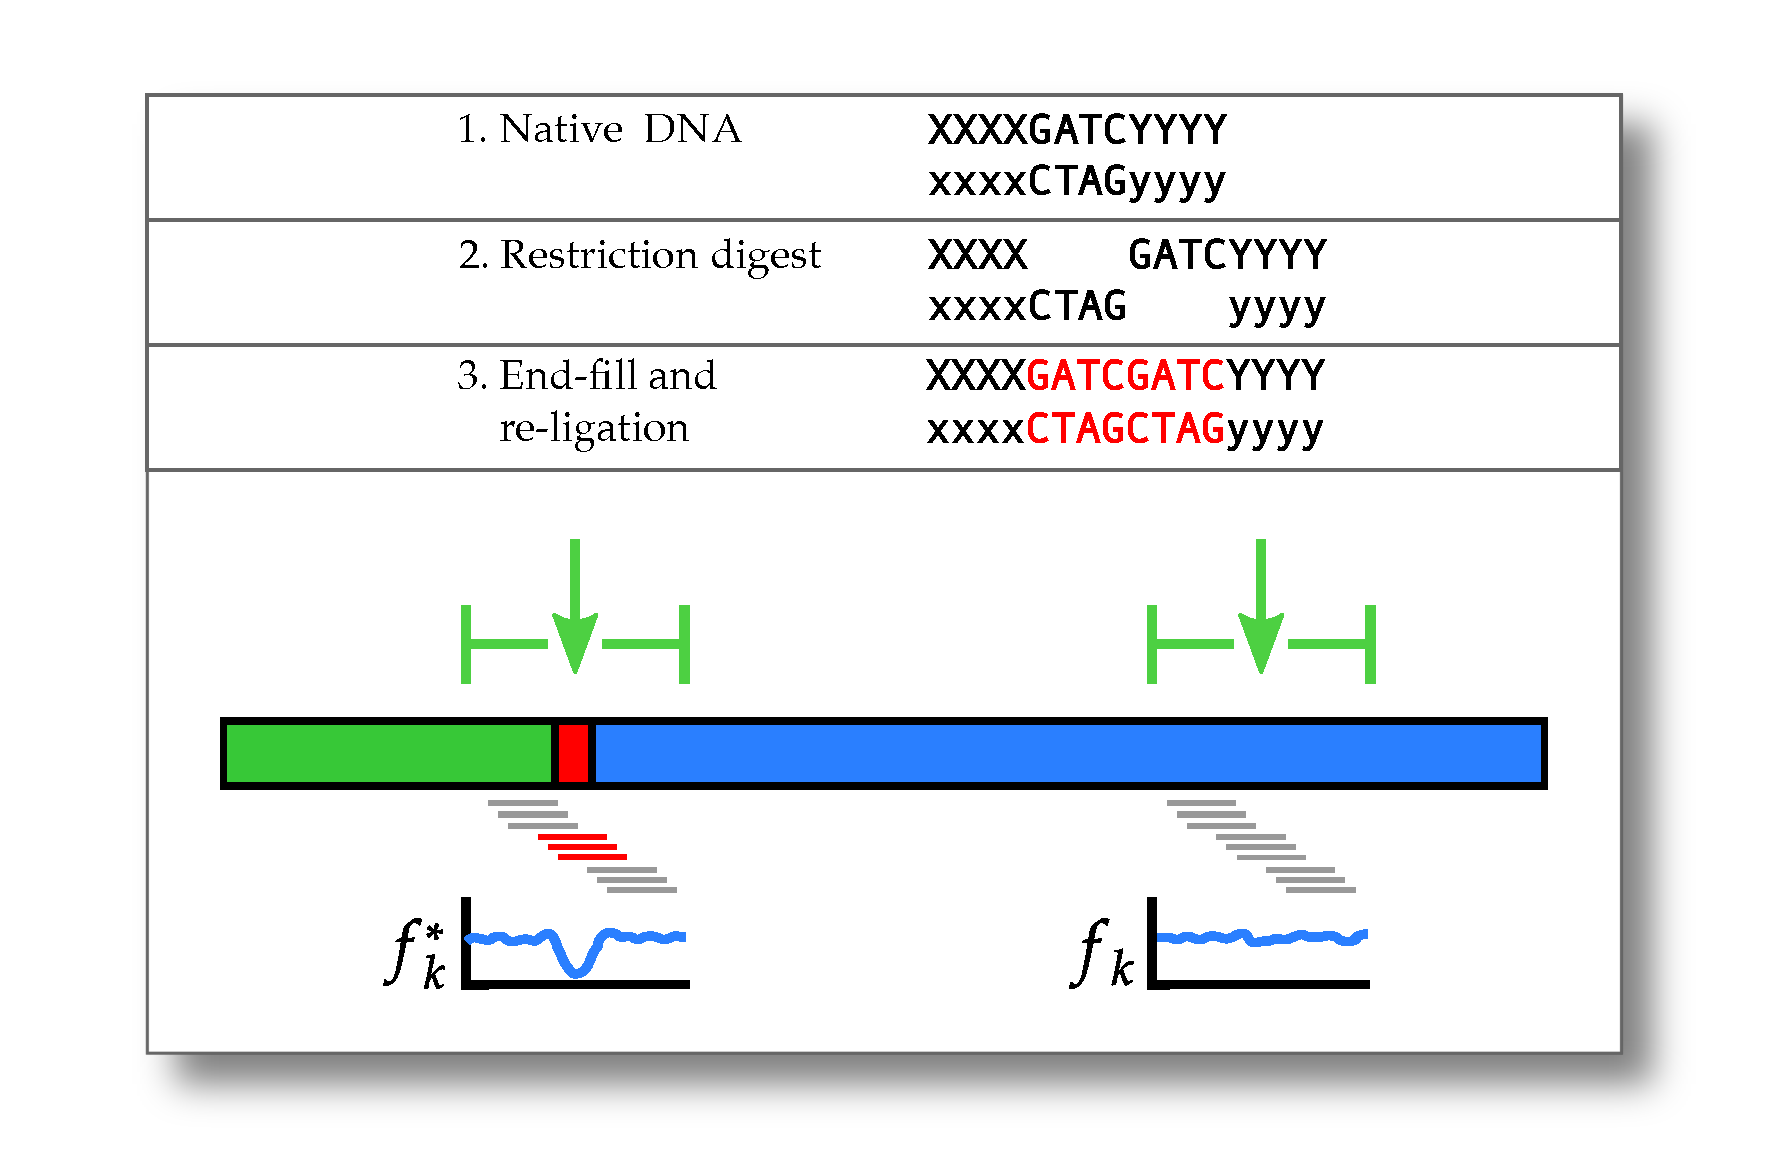
\includegraphics[width=0.85\linewidth]{method-figure-bigger.pdf}
\captionof{figure}{\color{Green} Hi-C proximity ligations produce chimeric DNA fragments, here stylised as the thick green and blue horizontal bars. At the ligation site (intervening red bar) a predictable DA is created. Our reference-free method exploits this introduced sequence. By sampling the frequency of local $k$-mers either side (small grey bars) and at the junction site (small red bars), we find the relative local frequency $f^*_k$ is characteristically lower than when the sampling is performed at native positions $f_k$.}
\label{fig:junction}
\end{center}\vspace{1cm}
\end{minipage}

\section*{Results and Discussion}

The reference-free method was validated using a simulated parameter sweep, where read-sets were simulated using sim3C \cite{DeMaere2018-gf} with \textit{E.coli} MG1655 (acc: GCF\_000005845.2) as the source genome. Ten replicates were generated for each step, where the sweep varied Hi-C signal content $[0.01 : 0.75]$, the number of available read-pairs $[10,000 : 500,000]$ and fragment length $[150 : 500]$, with read length fixed at 150bp. Agreement between the expected and predicted Hi-C fraction is very good at low signal levels, but an underestimation trend is evident as the simulated signal increases (fig. \ref{fig:simulation}). Although better agreement at high signal levels would be preferred, a tendency to conservative estimation would still lead to collecting sufficient depth were qc3C used to calibrate larger sequencing runs.

Three out eighteen real Hi-C read-sets from previous work \cite{Kadota2020-wd} were selected to demonstrate qc3C on real data (acc: DRR177159, DRR177161, DR177163). These three pilot sequencing runs represent a single labs effort to produce high quality Hi-C libraries from a single source genome using three different Hi-C protocols \cite{Kadota2020-wd}. Traditional referenced-based quality statistics for the libraries was estimated from 200,000 pairs and the resulting qc3C report visualised (fig. \ref{fig:multiqc}). Here, we can see that read acceptance rates varied between 50\% to 70\%, For accepted reads, valid Hi-C pairs varied between 70\% to 90\%. The breakdown of long-range pairs demonstrates how protocol changes can strongly influence what observations get collected. Lastly, the distribution of pair separation helps to further characterise each library, with two possessing significantly more density at larger separations.

\begin{minipage}{\linewidth}
\begin{center}\vspace{1cm}
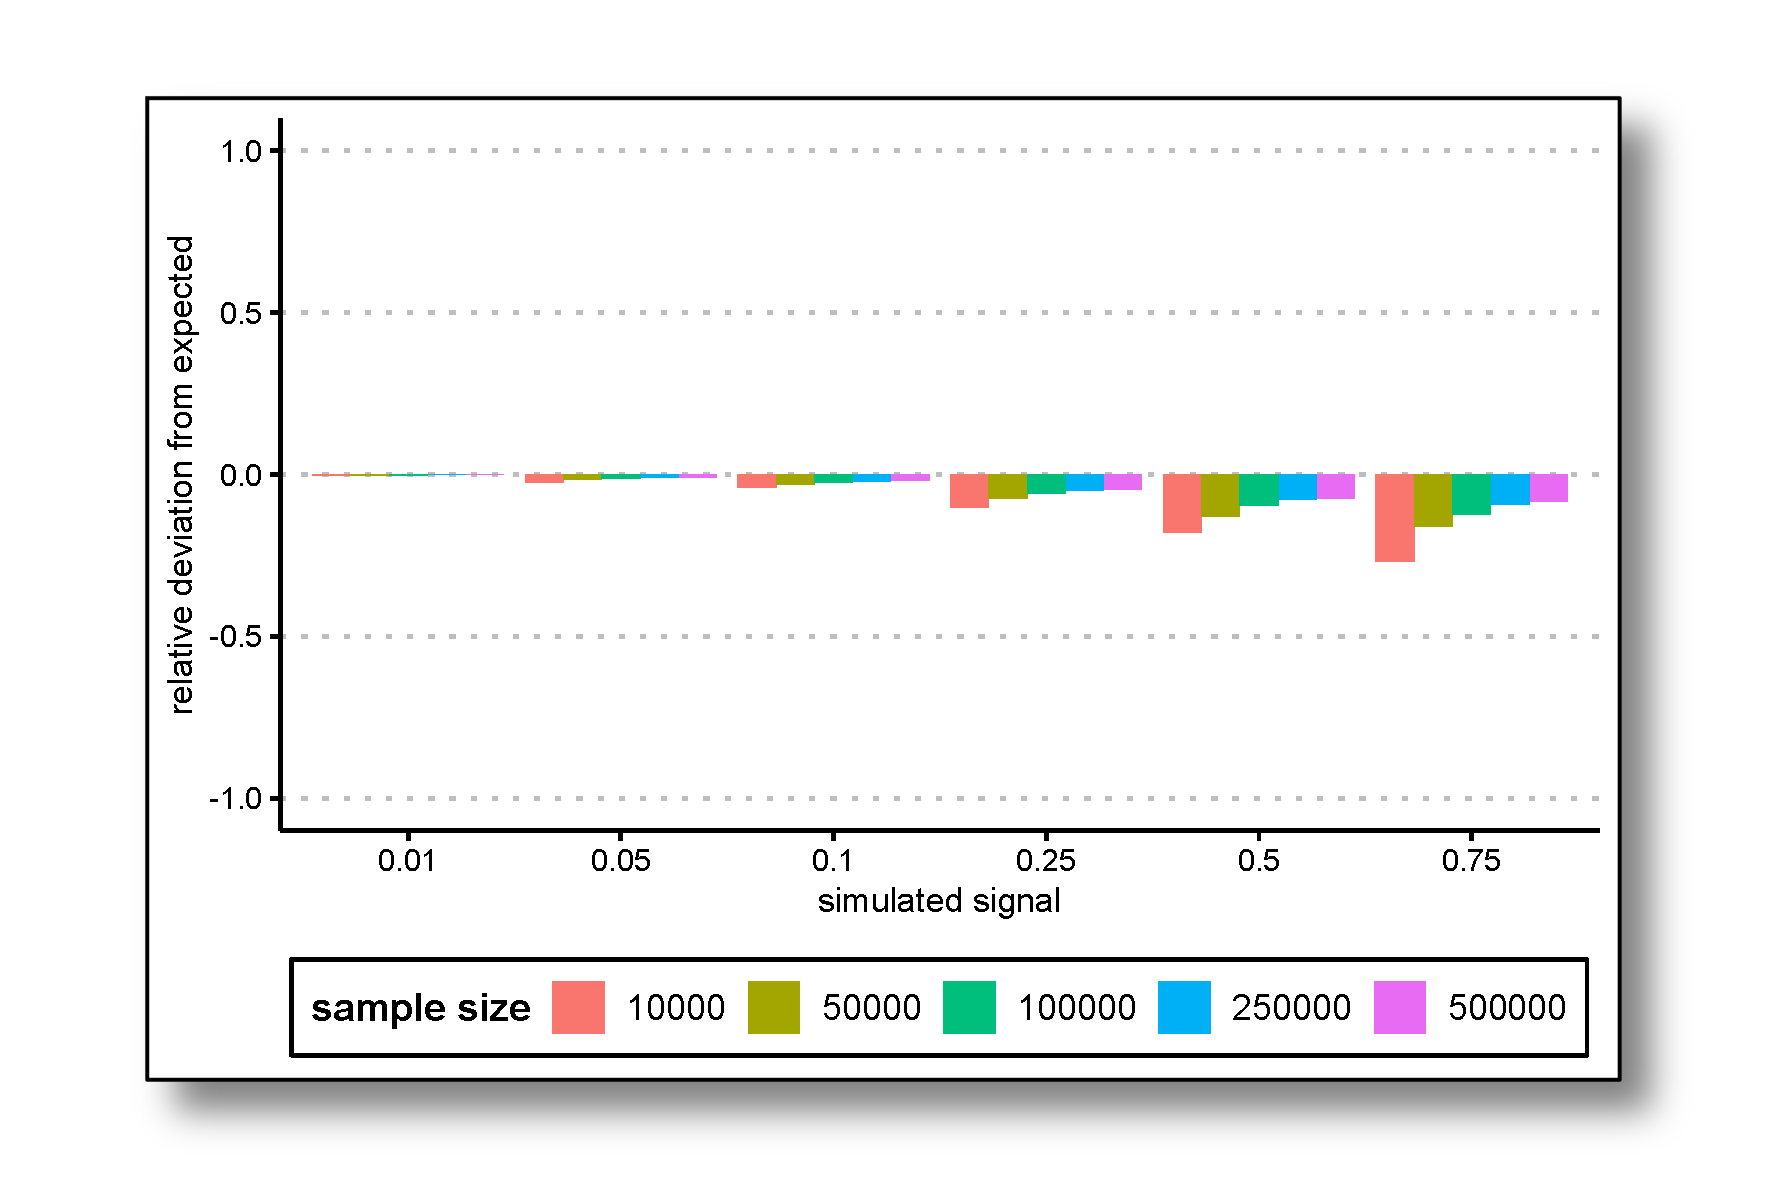
\includegraphics[width=0.85\linewidth]{simulation-plot.pdf}
\captionof{figure}{\color{Green} Reference-free estimation of Hi-C signal content for the simulated parameter sweep (fragment size = 250bp). The method is most accurate for low simulated signal. As the sample number of reads increases beyond 100,000 there are diminishing gains in precision and accuracy.}
\label{fig:simulation}
\end{center}\vspace{1cm}
\end{minipage}

\begin{minipage}{\linewidth}
\begin{center}
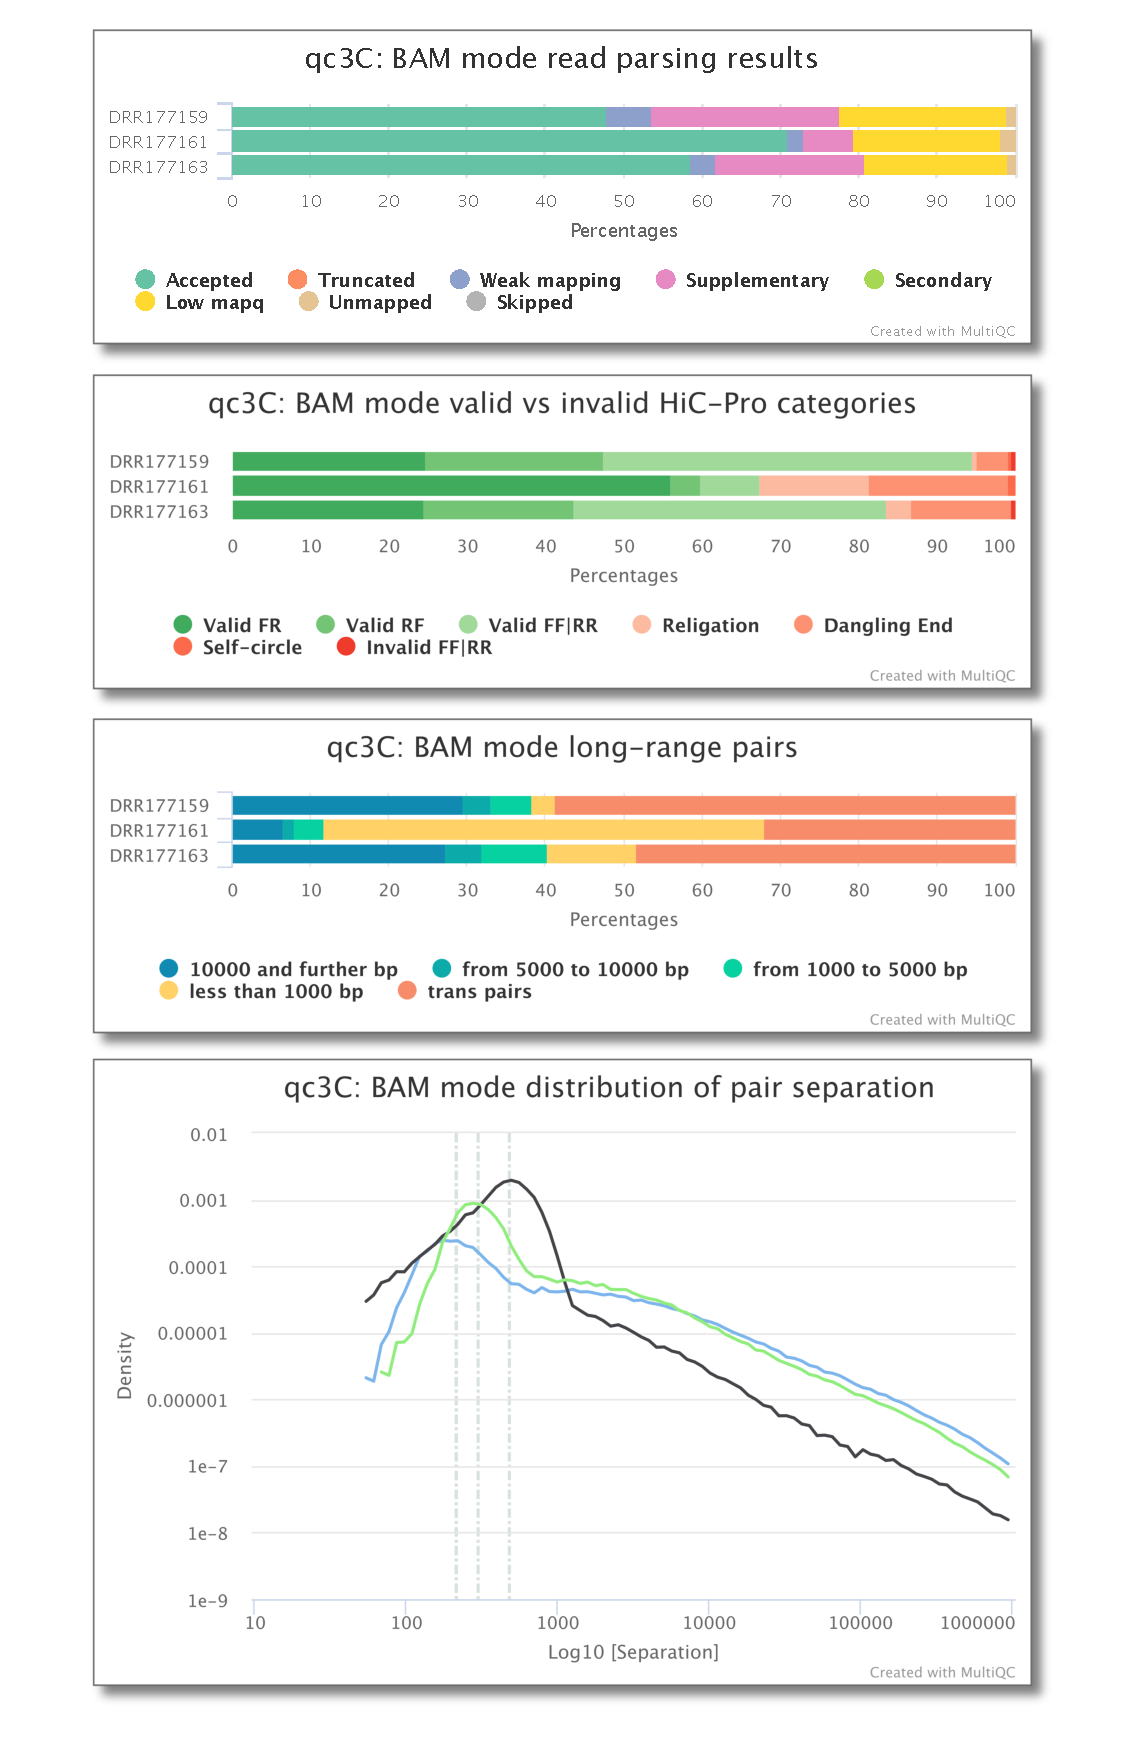
\includegraphics[width=0.85\linewidth]{multiqc-report.pdf}
\captionof{figure}{\color{Green} An example qc3C report of traditional referenced-based statistics for three real Hi-C libraries, as visualised by MultiQC. While these libraries derive from the same genomic source, each was generated using a different variation of the Hi-C protocol. In the lowest plot, the differing falloff of separation distance is evident, while dashed grey vertical bars mark qc3C mean size estimation of the unknown fragment portion.}
\label{fig:multiqc}
\end{center}
\end{minipage}

%----------------------------------------------------------------------------------------
%	REFERENCES
%----------------------------------------------------------------------------------------
\footnotesize
\nocite{*} % Print all references regardless of whether they were cited in the poster or not
\bibliographystyle{unsrt} % Plain referencing style
\bibliography{sample} % Use the example bibliography file sample.bib

%----------------------------------------------------------------------------------------
%	ACKNOWLEDGEMENTS
%----------------------------------------------------------------------------------------

\section*{Acknowledgements}
We would like to acknowledge our collaborators: Dr C Rinke, Prof AC McHardy, and Prof JA Eisen. This work was supported by ARC Discovery grant DP180101506. 
%----------------------------------------------------------------------------------------

\end{multicols}
\end{document}
